\section{NAX核心设计}
\subsection{目标和原则}
\subsubsection{设计目标}
在设计Token Economy时,为了达到激活生态的目的,每一项规则,无论是增发,销毁,使用场景等都需要符合一些基本原则和目标:

\begin{enumerate}[a.]
	\item 系统设计逻辑简洁有效
	\item 公平受益
	\item 正向激励,激励需要持续,规模适当
        \item 治理的有效凭证
        \item 具体持有价值
        \item 符合通缩模型,销毁与增发平衡
\end{enumerate}

\subsubsection{设计原则}
为了达到上述的设计目标,我们先从宏观经济模型中寻找一些可用的通用型经济规律。描述一个宏观经济体,为了促进经济体的繁荣发展,需要找到一些有意思的方向。从费雪公式中:

\begin{equation}
M * V = P * T
\end{equation}

\(M\)是Token数量,\(V\)是Token流通速度,\(P\)是Token价格,而\(T\)是系统内总交易额。

很好理解,等式两边其实算的都是以Token数量为计量的GDP。左边\(M * V\)是个数乘以流通速度等于GDP(Token计量),右边总GDP(法币计量)除以Token价格(法币计量)也等于GDP(Token计量)。

我们不难得出,增加Token的“持币价值”是最终有效促进经济体有效途径,然后增加Token的持有价值有如下方法:

\begin{enumerate}[a.]
	\item 增加质押、减少过多的流通量
	\item 提高非交易地址优势
	\item 增加持有NAS和NAX地址数
	\item 增加Token使用场景
\end{enumerate}

\subsection{NAX核心逻辑}
为了系统增发的公平性和有效性,NAX的增发场景只有通过Staking NAS获得。系统以每100,000高度作为一个周期,每个周期将根据当去的质押情况进行不同程度的增发。每周期过后,增发参数将以一程度衰减。一个直观的效果,经过一年之后,增发系数将会衰减到初始的一半左右。

公式如下:
其中,

\begin{enumerate}
   \item 第\(i\)期用户\(j\)获得的Token数量: \(K_{i,j}\)
   \item 第\(i\)期用户\(j\)的质押量: \(P_{i,j}\)
   \item 第\(i\)期用户\(j\)的质押时间: \(T_{i,j}\)
   \item 第\(i\)期初始总增发量:\(C_i\)
   \item 第\(i\)期增发比例: \(\lambda_i\)
   \item 相邻两期的增发衰减系数:$\mu$=0.983
   \item 质押池相比总流通量的比率:$\alpha$
\end{enumerate}

\begin{equation}
  K_{i,j} = \frac{P_{i,j} T_{i,j}}{\sum_j P_{i,j} T_{i,j}} \lambda_i C_i
\end{equation}

\begin{equation}
  \lambda_i = f(\sum_j P_{i,j} T_{i,j})
\end{equation}

\begin{equation}
  C_i = C_0 B^i
\end{equation}

同一个周期内,系统会根据质押数量以及相应的质押时间长短来分配增发的总量,以达到公平的效果,即质押数量越多,质押时间越长,所分配到的增发数量也会更多。该设计会达到以下博弈场景:
\begin{enumerate}
	\item 早期参与质押的用户,有更大的概率获得更多的系统增发
	\item 随着质押率增加,系统增发数量也会相应提高,以鼓励更多人加入质押
\end{enumerate}

\subsection{合约框架}
NAX是由一组合约组成,是在NRC20基础上扩展的合约组,并配有多签合约管理整个合约里的参数,详细如图1所示。

\begin{figure}[htbp]
    \centering
    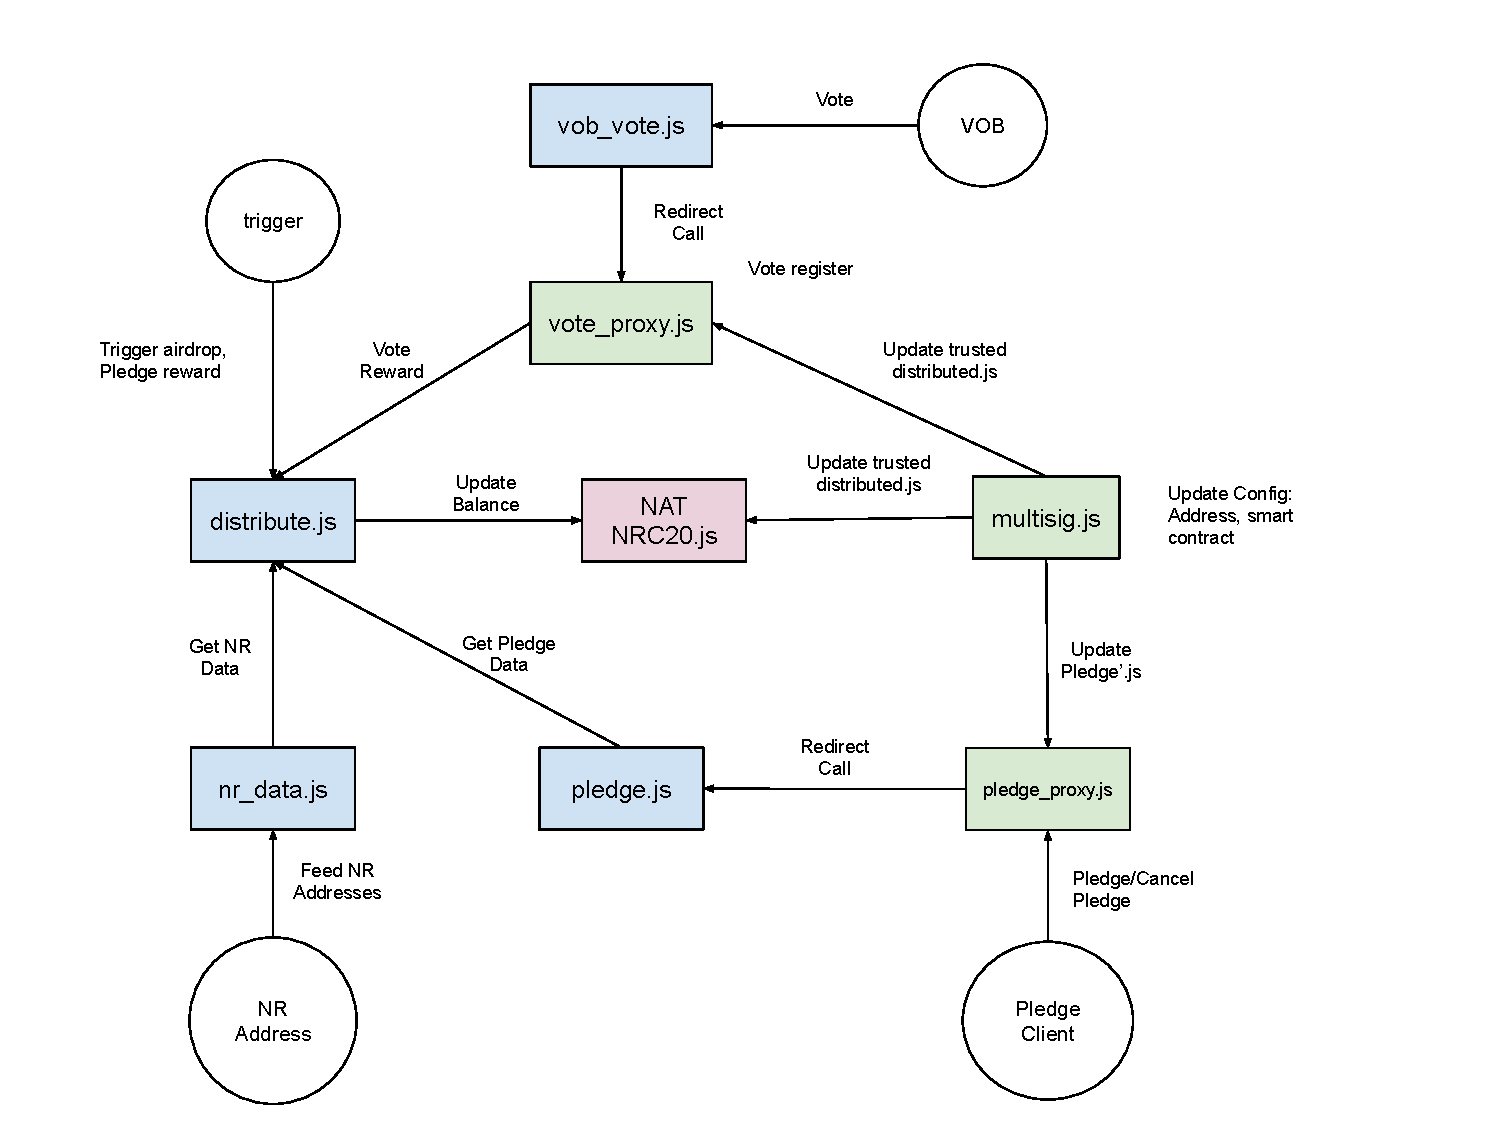
\includegraphics[width=1\textwidth]{../common/ch/nax.pdf}
    \caption{NAX 合约示意图(此图待更新) \label{fig:nax_framework}}
\end{figure}
